\chapter{Referencial Teórico}
\label{cap:Referencial Teórico}

% figuras estão no subdiretório "figuras/" dentro deste capítulo
\graphicspath{\currfiledir/figuras/}

%=====================================================

\section{PDP - Problema de Dobramento de Proteínas}

Proteínas são estruturas básicas, essenciais para vida e possuem incontáveis funções biológicas. Proteínas são sintetizadas pelos ribossomos seguindo um formato provido pelo mensageiro RNA (mRNA). Durante a síntese, as proteínas dobram (enovelam) em uma estrutura tridimensional única, conhecida como conformação nativa. Este processo é chamado: dobramento de proteínas (\textit{protein folding}). A função biológica de uma proteína depende da sua estrutura tridimensional.

As proteínas são polímeros compostos por sequências de aminoácidos (também chamados de resíduos) conectados linearmente por ligações peptídicas. Cada aminoácido é composto por um átomo central de carbono ($C\alpha$) conectado a um átomo de hidrogênio, um grupo amina, um grupo carboxila e uma cadeia lateral (\textit{side-chain}) a qual confere a cada aminoácido uma função distinta. Uma ligação peptídica é formada por dois aminoácidos quando o grupo carboxila de uma molécula reage com o grupo amina da outra. Este processo de agregação de aminoácidos é conhecido como desidratação pois libera uma molécula de água ($H_2O$) \cite{suzuki1986introduction}. Proteínas podem ser chamadas de cadeias polipeptídicas. Todos os aminoácidos tem o mesmo \textit{backbone} e se diferem dos outros apenas pela \textit{side-chain}, a qual pode ser um simples átomo de hidrogênio ou até um grupo heterocíclico complexo. A \textit{side-chain} define as propriedades físicas e químicas dos aminoácidos de uma proteína \cite{cox2013lehninger}.

%\subsection{Estrutura hierárquica e função das proteínas}

%As proteínas são tradicionalmente descritas em quatro níveis hierárquicos de %complexidade \cite{cox2013lehninger}:

%\begin{enumerate}
%	\item Estrutura primária: Nível de organização simples que visa representar apenas a sequência de aminoácidos de maneira linear. Representa apenas as ligações peptídicas entre os aminoácidos. (Colocar imagem?)
%	\item Estrutura secundária: Consiste em arranjos espaciais de regiões locais de uma proteína. Existem três estruturas secundárias importantes $\alpha$-hélices(PAULING; COREY; BRANSON, 1951a), $\beta$-folhas
%	(PAULING; COREY; BRANSON, 1951b) e turns (dobras) (LEWIS; MOMANY;
%	SCHERAGA, 1973).
%	$\alpha$-hélices é a forma mais comum de estrutura secundária. É uma estrutura semelhante a um bastão, onde o \textit{backbone} firmemente 
%	helicoide forma a parte interna do bastão, e as \textit{side-chains} se projetam para fora em uma disposição helicoidal(http://labs.icb.ufmg.br/lbcd/grupo1/alfa.html). $\beta$-folhas formada por 2 ou mais segmentos polipeptídicos da mesma molécula, ou de moléculas diferentes, dispostos lateralmente e estabilizados por pontes de hidrogênio entre os grupos $NH$ e $CO$.  (Benítez)
%	\textit{Turns} são compostos de três ou quatro aminoácidos e geralmente são localizados na superfície das proteínas formando dobras que redirecionam a cadeia polipeptídica para o interior da proteína. \textit{Turns} permitem que as proteínas sejam dobradas em estruturas altamente compactas.	As estruturas secundárias podem ser associadas formando estruturas super secundárias, chamadas de \textit{motifs} (BRANDEN; TOOZE, 1999; GRIFFITHS
%	et al., 2000; NÖLTING, 2006). Os \textit{motifs}  são padrões frequentemente encontrados em estruturas tridimensionais.
%\item Estrutura terciária: Trata do arranjo tridimensional dos aminoácidos que compõem uma proteína. Enquanto as estruturas secundárias são estabilizadas por pontes de hidrogênio, as estruturas terciárias são estabilizadas por iterações entre \textit{side-chains} hidrofóbicas e pontes de hidrogênio entre \textit{side-chains} polares. A estrutura terciária representa o dobramento de um polipeptídeo como resultado das interações entre as \textit{side-chains} dos aminoácidos que se encontram em diferentes regiões da estrutura primária.
%	\item Estrutura quaternária: É o nível de representação mais complexo e descreve o arranjo de duas mais subunidades polipeptídicas dobradas (estruturas terciárias) no espaço.
%A associação quaternária pode ser entre diferentes tipos de polipeptídeos (heterodímero)
%ou entre polipeptídeos idênticos (homodímero). Este nível de organização	descreve o número e posições relativas de subunidades em proteínas
%multiméricas. A Hemoglobina é um exemplo de proteína multimérica, pois é composta de duas cópias de polipeptídeos diferentes que interagem entre si. 

%\end{enumerate}

\section{Dobramento de proteínas}

É o processo em que cada cadeia polipeptídica é transformada em uma estrutura compacta que realiza alguma função biológica \cite{grantcharova2001mechanisms}. Estas funções incluem controle e regulação de processos químicos essenciais para os organismos vivos \cite{branden1999introduction}. A estrutura tridimensional mais estável é chamada de conformação nativa e é a qual permite que a proteína exerça corretamente sua função biológica \cite{lodish2000molecular, pedersen2000algorithms}.

Experimentos conduzidos por Anfinsen et al. \cite{sela1957reductive, anfinsen1972studies, anfinsen1961kinetics}, mostraram que as proteínas possuem apenas uma conformação nativa e que as informações essenciais que codificam a estrutura estão contidas na sequência de aminoácidos. A conformação tridimensional nativa é dada pela estrutura primária (sequência de aminoácidos) de uma proteína.

Muitas proteínas podem desnaturar por modificações no ambiente em que estão inseridas, conforme demonstrado por \cite{sela1957reductive, anfinsen1972studies, anfinsen1961kinetics}. Durante o processo de desnaturação as proteínas perdem sua forma nativa (desdobram) e, consequentemente, perdem sua função. O exemplo mais conhecido de desnaturação proteica é o da clara do ovo. A clara do ovo é composta por água e albumina. A albumina é uma proteína polar, portanto solúvel em 
água. Ao fritar ou cozinhar o ovo, eleva-se a temperatura, levando à desnaturação da albumina que, mesmo ao retornar à temperatura original, não consegue voltar à sua conformação nativa. Além de se desdobrarem é possível que ocorram erros de dobramento na formação das proteínas causando com que a proteína não exerça sua função biológica corretamente. Estudos tentam identificar causas para os erros de dobramento das proteínas pois muitas enfermidades são causadas pelo mal dobramento de proteínas como, por exemplo, mal de Alzheimer \cite{hutton2001analysis, selkoe2001clearing}, alguns tipos de câncer \cite{bell2002p53, dawson2003n, ishimaru2003fibrillar}, fibrose cística \cite{thomas1992altered}, arteriosclerose
\cite{ursini2002atherosclerosis}, mal de Parkinson \cite{mcnaught2001failure}, entre outras. 
Portanto, entender como o processo de dobramento de proteínas ocorre é de fundamental importância. Um dos objetivos comuns das ciências biológicas é caracterizar funcionalmente sequências de proteínas através da resolução de suas conformações nativas \cite{eswar2003tools}. Varias áreas da ciência, tais como Biologia, Medicina, Química Orgânica, realizam diferentes estudos das proteínas. Muitos destes estudos são voltados para o processo de dobramento das proteínas que pode sofrer alterações: tanto em como a conformação estará disposta no espaço, como ela estará agrupada e sobre sua má formação. Isto é muito relevante para estudos que visam à produção de medicamentos, suplementos alimentares, técnicas que manipulam o DNA, ou para formação de novos compostos proteicos sintéticos em laboratório \cite{devlin1998manual}. É importante mencionar que apesar do avanço na grande quantidade de proteínas que se tem conhecimento por conta de projetos de sequenciamento genômico, apenas uma pequena fração de estruturas tridimensionais é conhecida.

A cristalografia de raios-X e espectroscopia de RNM são os métodos experimentais mais poderosos para o estudo da estruturas de proteínas \cite{ilari2008protein} \cite{gobl2012application}. Entretanto estes métodos são altamente custosos tanto em esforços computacionais, de tempo e financeiros, e estão disponíveis apenas para algumas instituições.


Embora o conceito de dobramento de proteínas tenha surgido da área de biologia molecular, este problema é um problema interdisciplinar, o qual requer apoio de muitas áreas do conhecimento, e é considerado como um dos desafios atuais mais importantes da biologia e bioinformática \cite{nicosia2008generalized}. 

Na biologia computacional existem dois problemas que tratam sobre o dobramento de proteínas. São eles: problema de predição estrutura de proteínas (ou PSP - \textit{Protein Structure Prediction}), que trata de predizer a estrutura tridimensional (conformação) a partir de sua sequência (estrutura primária); e o problema de dobramento de proteínas (PDP ou PFP - \textit{Protein Folding Problem}), o qual trata da determinação dos passos/eventos que conduzem o dobramento a partir da estrutura primária até a conformação nativa \cite{lopes2008evolutionary}. Porém, na literatura, é encontrado ambos os termos sendo utilizados sem nenhuma distinção, normalmente se referindo apenas ao primeiro problema \cite{lopes2008evolutionary}.  

A ciência da computação desempenha um papel importante nisto, propondo e desenvolvendo modelos e soluções computacionais para o estudo de ambos os problemas PSP e PDP \cite{lopes2008evolutionary}. Muitas estratégias computacionais descrevem modelos de predição de estruturas de proteínas com diferentes níveis de detalhamento e complexidade mas que permitem uma representação fidedigna da estrutura tridimensional, sem perda de viabilidade computacional \cite{benitez2015algoritmo}. Dessa maneira  evita-se a obrigatoriedade do uso de métodos caros, aumentando a competitividade e auxiliando na consolidação de centros de pesquisa que desenvolvem estudos nesta área \cite{dill2000polymer}.

Acredita-se que a conformação nativa de uma proteína é a sua estrutura mais estável, adquirindo um estado de energia livre mínima, o que gerou a chamada hipótese da termodinâmica \cite{pedersen2000algorithms}. Os modelos de predição de estruturas normalmente são baseados nas leis da termodinâmica onde o problema é modelado como um problema de minimização da energia livre a respeito das possíveis conformações que uma proteína pode assumir \cite{benitez2015algoritmo}. A minimização da energia livre é assumida como o principal fator para a formação da estrutura da proteína. Portanto, a conformação nativa de uma proteína é dada por aquela que possuir o menor valor de energia livre.

Segundo \cite{pedersen2000algorithms}, um modelo computacional deve possuir algumas características:

\begin{itemize}
	\item Um conjunto de entidades que representam os átomos e as ligações entre eles. 
	\item Regras que definem as possíveis conformações.
	\item Uma função que seja computacionalmente factível, para calcular a energia livre das possíveis conformações.
\end{itemize}

A próxima subseção irá discorrer sobre alguns modelos de representação de estruturas de proteínas.

\section{Modelos de Representação de Proteínas}

Em suma existem duas classes de modelos de representação de estruturas de proteínas: analítico (também conhecido como \textit{all atom}) e discreto (chamado também de \textit{coarse-grained}). Os modelos analíticos possuem uma descrição detalhada da estrutura tridimensional incluindo informações de todos os átomos que constituem uma proteína. Já os modelos discretos descrevem as proteínas com um nível bastante reduzido de detalhes. Os modelos discretos recentemente ganharam maior interesse, por conta de dois fatores: a simulação de modelos analíticos nem sempre é computacionalmente possível e modelos discretos possibilitam simulações biologicamente relevantes com melhor aproveitamento  computacional \cite{benitez2015algoritmo}. Embora simulações utilizando modelos discretos ainda não possam ser consideradas tão preditivas quanto simulações analíticas, avanços notáveis têm: sido alcançados, referente ao uso de metodologias mais rigorosas e criação de algoritmos para melhor explorar o espaço de busca \cite{tozzini2005coarse}. Esta proposta irá descrever apenas os modelos discretos pois visa a utilização do modelo hidrofóbico polar (HP) 2D.

\subsection{Modelos Discretos}

Os modelos computacionais mais simples são os conhecidos como modelos de grade (\textit{lattice models}). Estes modelos consideram as estruturas de proteínas como um colar de esferas posicionado em uma grade. O grau de liberdade dos movimentos é restrito à estrutura da grade, que pode ser 2D (plano) ou 3D (espacial). Conformações válidas são aquelas que os aminoácidos adjacentes na sequência também são adjacentes na grade e cada aminoácido ocupe uma posição distinta na grade. Muitos modelos de grade têm sido propostos e aplicados ao PDP. Os modelos 2D-HP e 3D-HP são exemplos de modelos de grade.

\subsubsection{Modelo Hidrofóbico-Polar HP}
\label{subsubsection:modeloHP}

No modelo HP os aminoácidos são classificados em 2 tipos: Hidrofílicos (Polar) e Hidrofóbico. Consequentemente, uma proteína é representada por uma \textit{string} de caracteres definida por um alfabeto binário $\{H,P\}$. Este modelo considera que as interações entre aminoácidos hidrofóbicos (H) representam a contribuição mais importante para a energia livre de uma proteína. Portanto existe uma relação inversamente proporcional: quanto maior for a quantidade de interações hidrofóbicas (H-H), menor será a energia livre de uma proteína. Uma interação hidrofóbica (também conhecida como contato hidrofóbico) é definida como um par de aminoácidos do tipo H-H que não sejam consecutivos na sequência mas sejam adjacentes na grade.
Como dito anteriormente, uma conformação é dita válida quando nenhuma posição da grade é ocupada por mais que um aminoácido. Conformações inválidas possuem colisões entre os aminoácidos. Dada uma conformação válida para o modelo HP e $n$ o número de interações hidrofóbicas, a energia da conformação pode ser facilmente calculada utilizando a equação \ref{equation:energyHp}: 


\begin{align}
	\label{equation:energyHp}
	E(c) = n. (-1) 
	\
\end{align}


Quando uma proteína é dobrada na sua conformação nativa, os aminoácidos hidrofóbicos tendem a se agrupar no interior da estrutura, protegidos por aminoácidos polares posicionados no exterior. Dessa maneira, um núcleo hidrofóbico é formado em proteínas dobradas \cite{benitez2015algoritmo}. 
Embora simples, a estratégia computacional de buscar uma solução para o PDP utilizando modelo HP é considerada como um problema $NP$-completo \cite{atkins1999intractability, berger1998protein, crescenzi1998complexity}. O espaço de busca do modelo HP possui algumas características mencionadas na literatura \cite{bastolla1997testing, berger1998protein, crescenzi1998complexity, krasnogor1999protein, vendruscolo2000can} :

\begin{itemize}
	\item Elevada degenerescência.
	\item Espaço de busca multimodal.
	\item Muitas regiões com conformações inválidas.
\end{itemize}

A figura \ref{fig:exemploModeloHP} apresenta um exemplo para os modelos HP (2D e 3D). Os pontos pretos são aminoácidos do tipo H e os brancos são aminoácidos do tipo P. As linhas pontilhadas representam as interações hidrofóbicas.

%\begin{figure}[!htb]
%	\centering
%	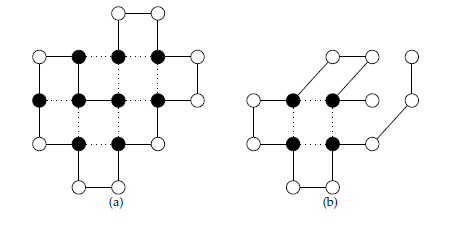
\includegraphics[scale=.9]{modeloHP/modeloHPExemplo.png}
%	\caption{Exemplos de representação de proteínas utilizando os modelos HP 2D-HP (a) e 3D-HP (b). \\ Fonte: Adaptado de \cite{benitez2015algoritmo}}
%	\label{fig:exemploModeloHP}
%\end{figure}


Diversos trabalhos aplicam algoritmos evolucionários e bio-inspirados ao problema de dobramento de proteínas utilizando o modelo HP. Uma decisão comum a todos trabalhos que utilizam o modelo HP é a de como representar as variáveis de entrada. Na literatura é possível encontrar basicamente três representações \cite{krasnogor1999protein, lopes2008evolutionary}: 

\begin{itemize}
	\item Coordenadas cartesianas: Este método  representa a posição de cada aminoácido utilizando suas coordenadas espaciais (x,y) no plano cartesiano 2D ou (x,y,z) no plano cartesiano 3D. Geralmente, sua utilização não é adequada para algoritmos baseados em população, pois estruturas idênticas ou semelhantes podem ter coordenadas totalmente diferentes  \cite{benitez2015algoritmo}; 
	\item Coordenadas internas: Nesta representação as conformações são representadas por conjuntos de movimentos que ditam como a estrutura final irá se parecer. Esta representação é a mais utilizada em abordagens com algoritmos evolucionários para o PDP \cite{benitez2015algoritmo}. Existem duas possibilidades de se representar conformações utilizando coordenadas internas:
	\begin{itemize}
		\item Coordenadas absolutas: Este tipo de coordenada é baseado na orientação do eixo da grade onde a conformação esta contida. No caso de uma grade bidimensional os possíveis movimentos são: $\{N,S,L,O\}$ ou norte,sul,leste e oeste. Já em uma grade 3D os possíveis movimentos são: $\{N,S,L,O,F,T\}$ que correspondem aos mesmos movimentos no caso 2D porém com dois movimentos a mais: para frente e para trás.
		\item Coordenadas relativas: Este tipo de representação define a posição de cada aminoácido da cadeia em relação ao movimento do seu predecessor. O conjunto de movimentos possíveis para a grade 2D é definido por $\{F,E,D\}$, que correspondem aos movimentos: frente (continuar no mesmo sentindo do aminoácido anterior), à esquerda e à direita. Em um cubo 3D, os possíveis movimentos são $\{F,E,D,C,B,\}$, possuindo dois movimentos a mais: para cima e para baixo. 
	\end{itemize}
	\item Matriz de distâncias: descreve a conformação de uma proteína através de uma matriz quadrada que representa a distância entre os aminoácidos. Este tipo de representação é raramente utilizado na literatura \cite{benitez2015algoritmo}.
\end{itemize}



\subsubsection{Outros Modelos}


Além do modelo HP, outros modelos simples em grade são utilizados para representar a estrutura de proteínas em outros estudos encontrados na literatura. Por exemplo:

\begin{itemize}
	\item Modelo PH (\textit{Perturbed Homopolymer}): Proposto por Shakhnovich et al. \cite{shakhnovich1993engineering}, as reações entre aminoácidos hidrofóbicos não são levadas em consideração, mas as interações entre aminoácidos do mesmo tipo são favorecidas, ou seja, H-H e P-P, desfavorecendo ligações H-P \cite{benitez2015algoritmo}.
	\item Modelo LPE (\textit{Lattice Polymer Embedding}): Modelo proposto por Unger e Moult \cite{unger1993finding}. A modelagem é feita a partir de uma sequência de aminoácidos, A = $a_1,...a_n$ atrelada a uma grade cúbica. Cada aminoácido possui um coeficiente de afinidade, definido para cada par $a_i,a_j (c(a_i,a_j))$. O objetivo da função de energia é minimizar o produto dos coeficientes pela distância entre os aminoácidos \cite{benitez2015algoritmo}.
	\item Modelo HP-TSSC (\textit{Hydrophobic-Polar Tangent Spheres Side Chain Model}): este modelo
	proposto por Hart et al. \cite{hart1997lattice} é baseado no modelo HP, porém não
	utiliza uma grade. Neste modelo a proteína é modelada via um grafo tridimensional, onde a cadeia lateral e o \textit{backbone}
	de cada aminoácido são esferas de mesmo raio \cite{benitez2015algoritmo}.
	\item Modelo CGE (\textit{Charged Graph Embedding}): Modelo descrito por Ngo et al. \cite{ngo1994protein}. Neste modelo, uma carga (\textit{charge}) é atribuída a cada
	resíduo. Entretanto, as conformações permitidas não são realistas \cite{benitez2015algoritmo}. 
	\item Modelo HPNX: modelo proposto por Bornberg-Bauer \cite{bornberg1997chain}. Divide
	os 20 aminoácidos em 3 classes: hidrofóbicos (H), positivos (P), negativos
	(N) e neutros (X). Este modelo, assim como o modelo HP, utiliza uma grade. Interações entre aminoácidos hidrofóbicos (H-H) representam
	interações de atração e diminuem a energia da conformação em 4,0,
	as interações entre positivos (P-P) e negativos (N-N) representam interações de repulsão e aumentam a energia livre em 1,0 e as interações entre N e P decrescem a energia em 1,0. O objetivo também consiste em minimizar a energia livre. Da mesma maneira que o modelo HP, quanto mais interações hidrofóbicas melhor será o dobramento. Porém este modelo não desconsidera o valor das demais interações \cite{benitez2015algoritmo}.
	\item Modelo HP-helicoidal (Helical-HP): este modelo proposto por Thomas e Dill \cite{thomas1993local} considera apenas uma grade bidimensional e inclui dois tipos de interação: interações não-locais através de energia de contatos hidrofóbicos e interações locais representadas por uma tendência à formação de a-hélices (chamada de propensão hélica) \cite{benitez2015algoritmo}.
	\item Modelo \textit{off-lattice} AB: este modelo proposto por Stillinger et al. \cite{stillinger1993toy} divide os aminoácidos em duas classes de acordo com sua polaridade: Hidrofóbicos (A) e Hidrofílicos (ou polares  B). Inicialmente, este modelo foi aplicado em duas dimensões (2D AB \textit{off-lattice}) e posteriormente aplicado para três dimensões (3D AB \textit{off-lattice}). Os aminoácidos não consecutivos interagem através de um potencial modificado de Lennard-Jones. Os ângulos de torsão entre ligações sucessivas também contribuem no cálculo da função de energia \cite{benitez2015algoritmo}.
	
\end{itemize}




\subsection{Considerações Finais}
\label{Problema de Dobramento de Proteínas:Consideracoes Finais}

Neste seção o problema de dobramento de proteínas foi apresentado e sua importância para biológica computacional, química orgânica e medicina. Também foi mencionado que existem diversos modelos para representar estruturas de proteínas. Cada modelo tem suas peculiaridades e considera interações diferentes. Não existe um modelo que represente de maneira real o dobramento de proteínas, pois se trata de um processo ainda não completamente compreendido pelos cientistas e pesquisadores. Os modelos propostos tem diferentes níveis de detalhe e complexidade. O modelo mais simples é o HP mas apesar da sua simplicidade se apresenta como um problema $NP$-completo. O modelo HP será utilizado nesta proposta por conta de sua simplicidade de implementação, assim como o baixo custo computacional para realizar simulações do cálculo de energia. Utilizando o modelo HP diferentes maneiras de representar as variáveis existem. Nesta dissertação será utilizada a representação relativa pois é mencionado na literatura que esta tem uma maior capacidade de guiar algoritmos de busca a melhores resultados.


%=====================================================

\section{AEs - Algoritmos Evolucionários}

Um algoritmo evolucionário (AE) é uma técnica de busca, altamente paralela, inspirada na teoria da seleção natural e reprodução genética de Charles Darwin. De acordo com a teoria de Darwin, a seleção natural irá favorecer os indíviduos que forem mais aptos, dessa maneira, estes indíviduos tem uma maior probabilidade
de reprodução. Indivíduos com mais descendentes tem uma chance maior de perpetuarem seus códigos genéticos nas gerações futuras. O código genético é a identidade de cada indivíduo e é representado por cromossomos. Estes princípios são utilizados na implementação de algoritmos computacionais, que procuram por soluções melhores para um dado problema, evoluindo uma população 
de soluções codificadas em cromossomos artificais -- estruturas de dados utilizadas para representar soluções factíveis para um dado problema \cite{pacheco1999algoritmos}.

De maneira geral, problemas reais de otimização possuem múltiplos objetivos a serem minimizados/maximizados e estão presentes em muitas áreas do conhecimento.
Para otimizar problemas multiobjetivos, dois ou mais objetivos são considerados os quais geralmenta são conflitantes. Para estes problemas é impossível encontrar uma
única solução ótima. Um conjunto de soluções é encontrado avaliando a dominância de Pareto \cite{pareto} entre as soluções. O objetivo principal é encontrar o conjunto  
de soluções que sejam não dominadas entre si. Uma solução domina outra, se e somente se, for melhor em pelos um dos objetivos, sem ser pior em qualquer outro.
Este conjunto de soluções constitui a fronteira de Pareto. Encontrar a fronteira real de Pareto é um problema NP-Completo \cite{fonseca2005tutorial}, dessa maneira,
o objetivo é encontrar uma boa aproximação da fronteira real.

Algoritmos Evolucionários Multi-Objetivos (AEMOs) são extensões de AEs para problemas multi-objetivos os quais aplicam
conceitos da dominância de Pareto para criar diferentes estratégias para evoluir e manter a diversidade das soluções.
Nesta dissertação foram explorados dois AEMOs: NSGAII \cite{deb2002fast} and IBEA \cite{zitzler2004indicator}.
%=====================================================

\subsection{NSGAII - Non-dominated sorting Genetic Algorithm II}

O algoritmo \ref{alg:nsgaII} apresenta o pseudo código do NSGAII. O algoritmo recebe como parâmetro $N$ o tamanho da população e $T$ o número máximo 
de avaliações. O algoritmo inicia criando uma população com tamanho $N$ chamada $P_0$. A população $P_0$ é classificada de acordo com aptidão 
e a relação de não dominância. A população $P_0$ é submitida ao operador de seleção: torneio binário para selecionar duas soluções que serão utilizadas
para gerar descendentes. Operadores de cruzamento e mutação são aplicados na soluções selecionadas gerando duas soluções distintas descendentes. 
Ao fim do processo de reprodução as soluções descendentes são avaliadas e adicionadas a população chamada $Q_0$.

Após esta estapa, $P_0$ e $Q_0$ são adicionadas em uma população auxiliar chamada $R$. Utilizando o conceito de não dominância, $R$ é ordenada 
criando fronteiras, onde cada solução da primeira fronteira não é dominada por nenhuma outra solução, já soluções da segunda fronteira são dominadas
apenas por soluções contidas na primeira fronteira, e assim por diante. Para cada fronteira, as soluções são avaliadas utilizando um mecanismo
de \textit{Crowding-Distance} as soluções com maiores valores irão ser adicionadas na população da próxima geração chamada $P_t$ onde $t$ é a
avaliação corrente.

Após criar e preencher $P_t$ com as soluções não dominadas de todas as fronteiras, a população $P_t$ é avaliada e então passa para um novo
torneio binário e reprodução, dessa maneira, iniciando uma novo ciclo do algoritmo.

\begin{algorithm}[htb!]
	\begin{algorithmic}[1]
		\State{$N \gets$ Population Size}
		\State{$T \gets$ Max evaluations}
		\State{$P_0 \gets CreatePopulation(N);$}
		\State{$CalculateFitness(P_0);$}
		\State{$FastNonDominatedSort(P_0);$}
		\State{$Q_0 \gets 0$}
		\While{$Q_0 < N$}
		\State{$Parents \gets BinaryTournament(P_0);$}
		\State{$Offspring \gets CrossoverMutation(Parents);$}
		\State{$Q_0 \gets Offspring$}
		\EndWhile
		\State{$CalculateFitness(Q_0);$}
		\State{$t \gets 0$}
		\While{$t < T$}
		\State{$R_t \gets P_t \cup Q_t;$}
		\State{$Fronts \gets FastNonDominatedSort(R_t);$}
		\State{$P_{t+1} \gets 0$}
		\State{$i \gets 0$}
		\While{$P_{t+1} + Front_i  < N$}
		\State{$CrowdingDistanceAssignment(Front_i);$}
		\State{$P_{t+1} \gets P_{t+1} \cup Front_i$}
		\State{$i \gets i + 1$}
		\EndWhile
		\State{$CrowdingDistanceSort(Front_i);$}
		\State{$P_{t+1} \gets P_{t+1} \cup Front_i[1:(N -P_{t+1})]$}
		
		\State{$Parents \gets BinaryTournament(P_{t+1});$}
		\State{$Q_{t+1} \gets CrossoverMutation(Parents);$}
		\State{$t \gets t +1$}
		\EndWhile
		\State{\Return{$P \gets$ Set of non-dominated solutions.}}
	\end{algorithmic}
	\caption{NSGAII}
	\label{alg:nsgaII}
\end{algorithm}


%=====================================================

\subsection{IBEA (Indicator-Based Evolutionary Algorithm)}

No contexto de otimização multiobjetiva, otimizar consiste em tentar encontrar a fronteira com uma boa aproximação da fronteira real de Pareto. 
Entretanto, não existe uma definição geral para "uma boa aproximação". Consequentemente, indicadores de qualidade vem sendo utilizados
para avaliar a qualidade da aproximação de fronteiras. O indicador \textit{hypervolume} é um exemplo de indicador utilizado para avaliação e comparação 
das fronteiras.

No algoritmo IBEA, indicadores de qualidade são	utilizados para avaliar o conjunto de soluções não dominadas \cite{figueiredo2013algoritmo}.
Para utilizar o IBEA, é necessário definir qual indicador será utilizado para associar cada solução a um valor scalar. Um dos indicadores bastante utilizados
em conjunto com IBEA é o \textit{hypervolume} por conta da sua capacidade de avaliar a convergência e a diversidade do espaço de busca ao mesmo \cite{ishibuchi2008evolutionary}.

\begin{equation} \label{eq:ibea_fitness}
F(x_i) = \sum_{x_j \in (P-x_i)} {-e^\frac{-I_{Hy}(x_j,x_i)}{k}}
\end{equation}

A equação de \textit{fitness} do IBEA é apresentada pela equação \ref{eq:ibea_fitness} e é utilizada para calcular a contribuição de uma dada solução
para o valor do indicador referente a população, onde $k$ é um fator escalar dependente do $I_{Hy}$, o qual representa o indicador de qualidade sendo utilizado.
O valor $F(x_i)$ corresponde à perda de qualidade da aproximação, da fronteira real de Pareto, se a solução $x_i$ for removida da população \cite{figueiredo2013algoritmo}.





\section{Exemplo de figura}

A forma sugerida para incluir figuras em um documento \LaTeX\ é importá-las usando o pacote \texttt{graphicx}. Como formatos gráficos sugere-se:

\begin{itemize}

\item Formatos \emph{raster}, como PNG (\emph{Portable Network Graphics}) ou JPG (\emph{Joint Photographic Experts Group}) para fotografias; procure usar uma resolução de ao menos 150 dpi (\emph{dots per inch}).

\item Formatos vetoriais, como PDF (\emph{Portable Document Format}) ou EPS (\emph{Extended PostScript}) para diagramas e gráficos\footnote{NUNCA use JPG ou GIF para desenhos vetoriais, pois o resultado final geralmente fica borrado.}.

\end{itemize}

A maior parte das ferramentas permite exportar figuras nesses formatos (a figura do exemplo foi produzida com o \emph{Inkscape}, um programa livre multiplataforma). A figura \ref{fig:comun-intra-inter} mostra um exemplo de inclusão de figura em PDF.

% exemplo de inserção de figura
\begin{figure}[!htb]
\centering
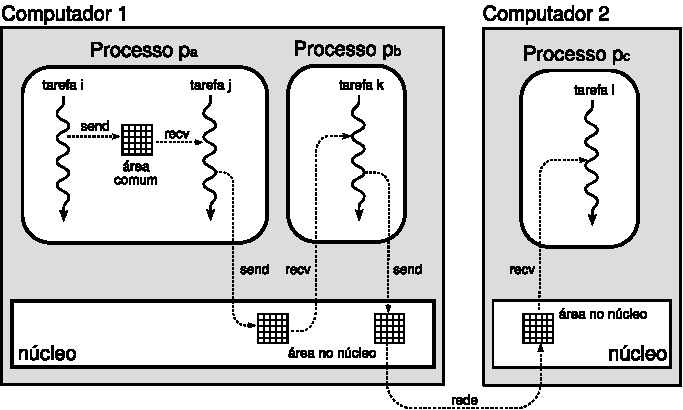
\includegraphics[width=12cm]{exemplo-figura.pdf}
\caption{Comunicação inter-processos.}
\label{fig:comun-intra-inter}
\end{figure}

Para mais informações consulte \cite{goossens93}.

%=====================================================

\section{Exemplo de tabela}

Tabelas são elementos importantes de um documento. No \LaTeX\ as tabelas podem ser objetos flutuantes (definidas no ambiente \texttt{table} e referenciadas por números usando \texttt{label} e \texttt{ref}) ou objetos fixos simples, criados pelo ambiente \texttt{tabular}. A tabela \ref{tab:modelos} é um exemplo de tabela flutuante, cuja posição no texto pode variar em função das quebras de página.

\begin{table}[!htp]
\centering
\caption{Os 16 modelos centrais do UCON$_{\mathrm{ABC}}$}
\label{tab:modelos}
\begin{tabular}{|c|cccc|}
\cline{2-5}
\multicolumn{1}{c|}{}& 0 (imutável) & 1 (\emph{pre-update}) & 2 (\emph{on-update}) & 3 (\emph{pos-update}) \\
\hline
\texttt{preA} & \textbullet & \textbullet & -- & \textbullet \\
\hline
\texttt{onA} & \textbullet & \textbullet & \textbullet & \textbullet \\
\hline
\texttt{preB} & \textbullet & \textbullet & -- & \textbullet \\
\hline
\texttt{onB} & \textbullet & \textbullet & \textbullet & \textbullet \\
\hline
\texttt{preC} & \textbullet & -- & -- & -- \\
\hline
\texttt{onC} & \textbullet & -- & -- & -- \\
\hline
\end{tabular}
\end{table}

%=====================================================

\section{Exemplo de equação}

Equações destacadas devem ser numeradas como mostra a equação \ref{eq:relatividade}:

\begin{equation}
E = m \times c^2
\label{eq:relatividade}
\end{equation}

%=====================================================

\section{Exemplos de código-fonte}

Códigos-fonte podem ser produzidos de forma simples através do ambiente \texttt{verbatim}, como mostra este exemplo:

\begin{footnotesize}
\begin{verbatim}
#include <stdio.h>

int main (int argc, char *argv[])
{
   int i ;                           // uma variavel local

   for (i=0; i< 100; i++)            // um laço for
      printf ("i vale %d\n", i) ;    // uma saída na tela
}
\end{verbatim}
\end{footnotesize}

No entanto, é preferível usar pacotes especializados para a edição ou inclusão de códigos-fonte, como o pacote \texttt{listings}. Eis um exemplo de código-fonte escrito com esse pacote:

% exemplo de código-fonte definido no próprio texto

\begin{lstlisting}
#include <stdio.h>

int main (int argc, char *argv[])
{
   int i ;                           // uma variável local

   for (i=0; i< 100; i++)            // um laço for
      printf ("i vale %d\n", i) ;    // uma saída na tela
}
\end{lstlisting}

Esse pacote também permite incluir códigos-fonte de arquivos externos. Eis um exemplo:

% exemplo de código-fonte incluso

\lstinputlisting{2-fundam/exemplo.c}

%=====================================================

%\section{Exemplo de algoritmo}
%
%Os pacotes \texttt{algorithm} e \texttt{algorithmic} permitem formatar algoritmos facilmente. Eis um exemplo:
%
%\begin{algorithm}[H]
%\caption{Ações de $s_i$ ao encerrar um ciclo:}
%\label{alg:on-period-ending}
%\begin{small}
%\begin{algorithmic}[1]
%\FORALL{$x \in \mathcal{K}_i$}
%  \STATE{$\mathit{banned}_i(x) \gets$ FALSE}
%  \STATE{$mi_i(x) \gets 0$}
%  \STATE{$mm_i(x) \gets 0$}
%  \STATE{$\mathit{age}_i(x) \gets \mathit{age}_i(x) + 1$}
%  \IF{$\mathit{age}_i(x) = \mathit{age}_\mathit{max}$}
%     \STATE{$\mathcal{K}_i \gets \mathcal{K}_i - \{x\}$}
%     \COMMENT{``esquece'' do servidor $x$}
%     \STATE{remove as informações locais sobre $x$}
%     \STATE{envia $\mathit{notify}(x,\mathit{undef})$ ao grupo de confiança $\mathcal{T}_i$}
%  \ENDIF
%\ENDFOR
%\end{algorithmic}
%\end{small}
%\end{algorithm}
 
%=====================================================

\section{Conclusão}

Todo capítulo (com exceção da introdução e da conclusão) deve encerrar com uma pequena conclusão local, resumindo os tópicos apresentados no capítulo e preparando o leitor para o próximo capítulo (exceto se esse for a conclusão geral). Caso o capítulo tenha apresentado resultados obtidos pelo próprio autor, estes devem ser sucintamente relembrados aqui.

%=====================================================
